\documentclass{llncs}

\usepackage{url}
\usepackage{graphicx}
\usepackage{listings}
\usepackage{verbatim}
\usepackage[lined,linesnumbered,algochapter]{algorithm2e}
\usepackage{tikz}
\usetikzlibrary{arrows,automata}
\usepackage{xspace}

\usepackage{ngerman}
\usepackage[ngerman, english]{babel}
\usepackage{bibgerm,cite}       % Deutsche Bezeichnungen, Automatisches Zusammenfassen von Literaturstellen
\usepackage[ngerman]{varioref}  % Querverweise

\setcounter{secnumdepth}{2}
\setcounter{tocdepth}{3}

% define custom macros for specific formats or names
\newcommand{\uml}[1]{\texttt{#1}}
\newcommand{\cd}{\textsf{Class Diagram}}

\begin{document}

\pagenumbering{roman}

\title{Code Generation by Object Observation - an Evaluation\footnote{This work has been created in the context of the course ``Advanced Model Engineering'' (188952) in SS13.}}


%&&&&&&&&&&&&&&&&&&&&&&&&&&&&&&&&&&&&&&&&&&&&&&&&&&&&&&&&&&&&&&&&&&&&&&&&
% Name and address of the author
%&&&&&&&&&&&&&&&&&&&&&&&&&&&&&&&&&&&&&&&&&&&&&&&&&&&&&&&&&&&&&&&&&&&&&&&&

\author{Sebastian Geiger\inst{1}, Sebastian Kerekes\inst{2}, Michael Kraxner\inst{3}, and Martin Lackner\inst{4} }

\institute{Favoritenstrasse 9-11, 1040 Wien \\ \email{sbastig@gmx.net} \\ MatrNr.: 
\and 
Favoritenstrasse 9-11, 1040 Wien \\ \email{contact@sebastiankerekes.com} \\ MatrNr.: 
\and
Favoritenstrasse 9-11, 1040 Wien \\ \email{michael.kraxner@gmail.com} \\ MatrNr.: 9925916
\and
Favoritenstrasse 9-11, 1040 Wien \\ \email{lackner.martin@gmail.com} \\ MatrNr.: 0927551
}



%&&&&&&&&&&&&&&&&&&&&&&&&&&&&&&&&&&&&&&&&&&&&&&&&&&&&&&&&&&&&&&&&&&&&&&&&
% Example for more than one authors
%&&&&&&&&&&&&&&&&&&&&&&&&&&&&&&&&&&&&&&&&&&&&&&&&&&&&&&&&&&&&&&&&&&&&&&&&
%\author{Max Mustermann\inst{1} and Matthias Mustermann\inst{2}}

%\institute{Musterweg 12/3/7, 1040 Wien \\ \email{mustermann@tuwien.ac.at} \\ MatrNr.: 0748549
%\and
%Mustergasse 54/4/3, 1030 Wien \\ \email{matthias@tuwien.ac.at} \\ MatrNr.: 0426553
%}

\maketitle

\begin{abstract}
 \dots
This paper evaluates possibilities and limitations of code generation by object observation. 
% This abstract summarizes the content of this paper in about 70 to 150 words.
 \dots
\end{abstract}

%&&&&&&&&&&&&&&&&&&&&&&&&&&&&&&&&&&&&&&&&&&&&&&&&&&&&&&&&&&&&&&&&&&&&&&&&
% Table of contents
% Activate or deactivate this according to the guideline instructor
%&&&&&&&&&&&&&&&&&&&&&&&&&&&&&&&&&&&&&&&&&&&&&&&&&&&&&&&&&&&&&&&&&&&&&&&&
\tableofcontents
%\thispagestyle{plain}
\newpage

\pagenumbering{arabic}

\section{Introduction}
In the last decade model driven engineering has devop  \dots
% This document is intended as a template and guideline and should support the author in the course of creating a seminar paper. Assessment criteria comprise the quality of the theoretical and/or practical work as well as structure, content and wording of the written seminar paper. Careful attention should be given to the basics of scientific work (e.g., correct citation).


\section{Semantics}
\label{sec:semantics}
Any (model) language is defined by its syntax, in this context a metamodel, and its semantics, the meaning of each element in the metamodel. We can distinguish between the static and the dynamic semantics. The static semantics defines structural properties of model elements in a metamodel (for further reading see~\cite{jour:10}~\cite{jour:3}), and the dynamic semantics regards to the execution of such models and its behavior~\cite{jour:3}. For our work we are interested in the dynamic semantics.

\subsubsection{Dynamic Semantics}
The dynamic or execution semantics defines the behavior under execution of models. This can be done in many ways, e.g., the semantics of UML is defined in OCL and natural language. A more sophisticated way which is seen very often in practice is either to use code generators to generate compilable source code, or to provide an interpreter which can process the models directly. But this approach is only feasible if the semantics is defined formally. Otherwise it would be too error prone, time-consuming and very costly if this would be done by manually studying and exploring the models~\cite{jour:3}.

We can distinguish between four different "semantic description styles" to define the semantics of a model formally~\cite{jour:3}~\cite{jour:10}:
\begin{description}
\item [Denotational] \hfill \\
This semantic provides a mapping between mathematical functions and model specific language constructs. E.g., it maps the keyword "-" to the subtraction function on natural numbers.
\item [Axiomatic] \hfill \\
This semantic provides a mapping between logical rules and model specific language constructs. E.g., stating that two arguments of a function "-" produces an output with the same type of the two arguments.
\item [Translational] \hfill \\
This semantic provides a mapping between the elements of a original model and model elements of a language where the semantics is already formally defined. The mapping is done by model transformation and can be used if the semantics of the source and the target models are closely correlated. Due to the fact, that the model transformation is done on the syntax level it is not guaranteed that the semantic of the final model behaves as desired. You also have to have an in-depth knowledge of both model languages and use multiple frameworks to achive good results.
\item [Operational] \hfill \\
This semantics describes how model constructs are executed on an abstract machine. It describes the effect of the computation and how the computation is produced.
\end{description}

Another approach to define the semantics is to "weave behavior" into the abstract syntax by a meta-language. On this approach the behavior of an operation is specified inside the body of the operation on the meta level. E.g., Kermata uses this approach by extending its abstract meta-layer with an imperative action language~\cite{jour:4}.

The last approach we will mention here is to define semantics with "Rewrite Rules". A system consits of rewrite rules and each rewrite rule has a left- and a right-hand side. When executing a model the system takes an model element, looks if such a model element occurs on the left-hand side of a rule and replaces it with the right-hand side if such a configuration is found~\cite{jour:4}.

\section{Code Generation by Observation vs. Compilation}
\label{sec:observationcompilation}
As already mentioned in~\ref{sec:semantics} there are two possible ways to execute models. Either you can generate code for your model, compile and execute it then, or you can make use of a model interpretor (execution engine), or you can combine these two methods. At the second possibility there must exist a kind of virtual machine which executes the model and fires events which can be catched, and therefor code can be generated by observating these events.

\subsubsection{Interpretation}
On interpretation, instance code is written for each model element which has be done once by the developer of the interpretation engine. Whenever a model is executed by the interpretation engine it analyzes the given model element at run-time and chooses the right instance implementation which will be executed then. E.g., if you have an user defined EClass in your model the interpretation engine stores this class in a hashmap with all its properties~\cite{misc:mdd}~\cite{jour:5}.

\begin{description}
\item [Advantages of Model Interpretation] \hfill \\
Here are some of the advantages of model interpretation~\cite{misc:mdd}.
\begin{description}
\item [Enable Debugging] \hfill \\
When models are interpreted it is possible for developers to debug thru the models. This can be very helpfull on complex models.
\item [Faster Changes] \hfill \\
Models can be faster changed because there is no need to regenerate, rebuild, retest and redeploy the whole model.
\item [Changes at Runtime] \hfill \\
Models can be changed during runtime without stopping the running application.
\end{description}

\end{description}

\subsubsection{Compilation}
If you are using code generators you have to write a compiler component which can deal with any model element of your meta-model. You have to generate code for every model element and compile it for a specific model. At run-time the model element logic is inside the instance code. E.g., if you have an user defined EClass in your model you can use a template based code generation approach where for each EClass in your model a java class is generated and filled with the corresponding properties~\cite{misc:mdd}~\cite{jour:5}.

\begin{description}
\item [Advantages of Compilation] \hfill \\
Here are some of the advantages of compilation~\cite{misc:mdd}.
\begin{description}
\item [Additional Checks] \hfill \\
Code which will be generated need to be compiled. The compiler will check the code for errors which is not be done by an interpretor.
\item [Architecture Independence] \hfill \\
If you are using an interpretor you have always to follow your own architecture. When using code generation you can suite the architecture of the code for the customer needs.
\item [Easier to Understand] \hfill \\
Generated code is easier to understand, you can follow the code line by line and understand the behavior exactly. On model interpretation you have to understand the implementation of the interpretor and also the semantics of the model.
\end{description}
\end{description}

\subsubsection{Resume}
It depends on the use case, on the developers skills and of the domain if you are using an interpreator or code generators. There are advantages and disadvantages on both approaches. In the next chapters we will take a closer look on both approaches and discuss the advantages and disadvantages in detail.

\section{Related work}

 recent developments  \dots Executable UML, 

\subsection{fUML}
\subsection{xMOF}
\subsection{xtend}
XXX really ???

\subsection{Code Generation with xtend}


\subsection{Code Generation by Object Observation}



\section{Evaluation}

%
%
%For working with LaTeX you can take advantage of a variety of books and free introductions and tutorials on the internet. A competent contact point for LaTeX beginners is the LaTeX Wikibook, which is available under \url{http://en.wikibooks.org/wiki/LaTeX}. 
%
%The following sections give examples of the most important LaTeX environments and commands.
%
%\subsection{Tables}
%
%Tables have to be realized with the help of the \textit{table} environment. Tables shall be sequentially numbered for each chapter and described in terms of a short caption (cf. Table~\ref{tab:diplomaseminar}).
%
%\begin{table}[htb]
%	\centering
%	\begin{tabular}{|l|c|c|}
%		\hline \textbf{Name} & \textbf{Date} & \textbf{Title} \\
%		\hline
%		\hline Mustermann Adam  & 18.5   & T1    \\
%		\hline Musterfrau Eva  & 22.6   & T2    \\
%		\hline
%	\end{tabular}
%	\caption{Seminar for Master Students}
%	\label{tab:diplomaseminar}
%\end{table}
%
%
%\subsection{Figures}
%
%Like tables, figures shall be sequentially numbered for each chapter and described in terms of a short caption). You could either produce your drawings directly inside Latex using PSTricks\footnote{\url{http://tug.org/PSTricks}}, Tikz\footnote{\url{http://sourceforge.net/projects/pgf}}, or any set of macros dedicated to your requirements (cf. Figure~\ref{fig:samplefigure_tikz}). Alternatively, you may include figures prepared in external tools (cf. Figure~\ref{fig:samplefigure_pdf}). Note, to ensure high quality printing, all figures must have at least 300 dpi.
%
%\begin{figure}
%	\centering
%	\begin{tikzpicture}[->, auto, node distance=2.8cm, semithick]
%	  \node[initial, state] (1)		 {$S_1$};
%	  \node[state] 		(2) [right of=1] {$S_2$};
%	
%	  \path (1) edge [bend left]  node {0} (2)
%		(1) edge [loop above] node {1} (1)
%		(2) edge [bend left]  node {0} (1)
%		(2) edge [loop above] node {1} (2);
%	\end{tikzpicture}
%	\caption{Sample figure}
%	\label{fig:samplefigure_tikz}
%\end{figure}
%
%\begin{figure}[tb]
%	\centering
%	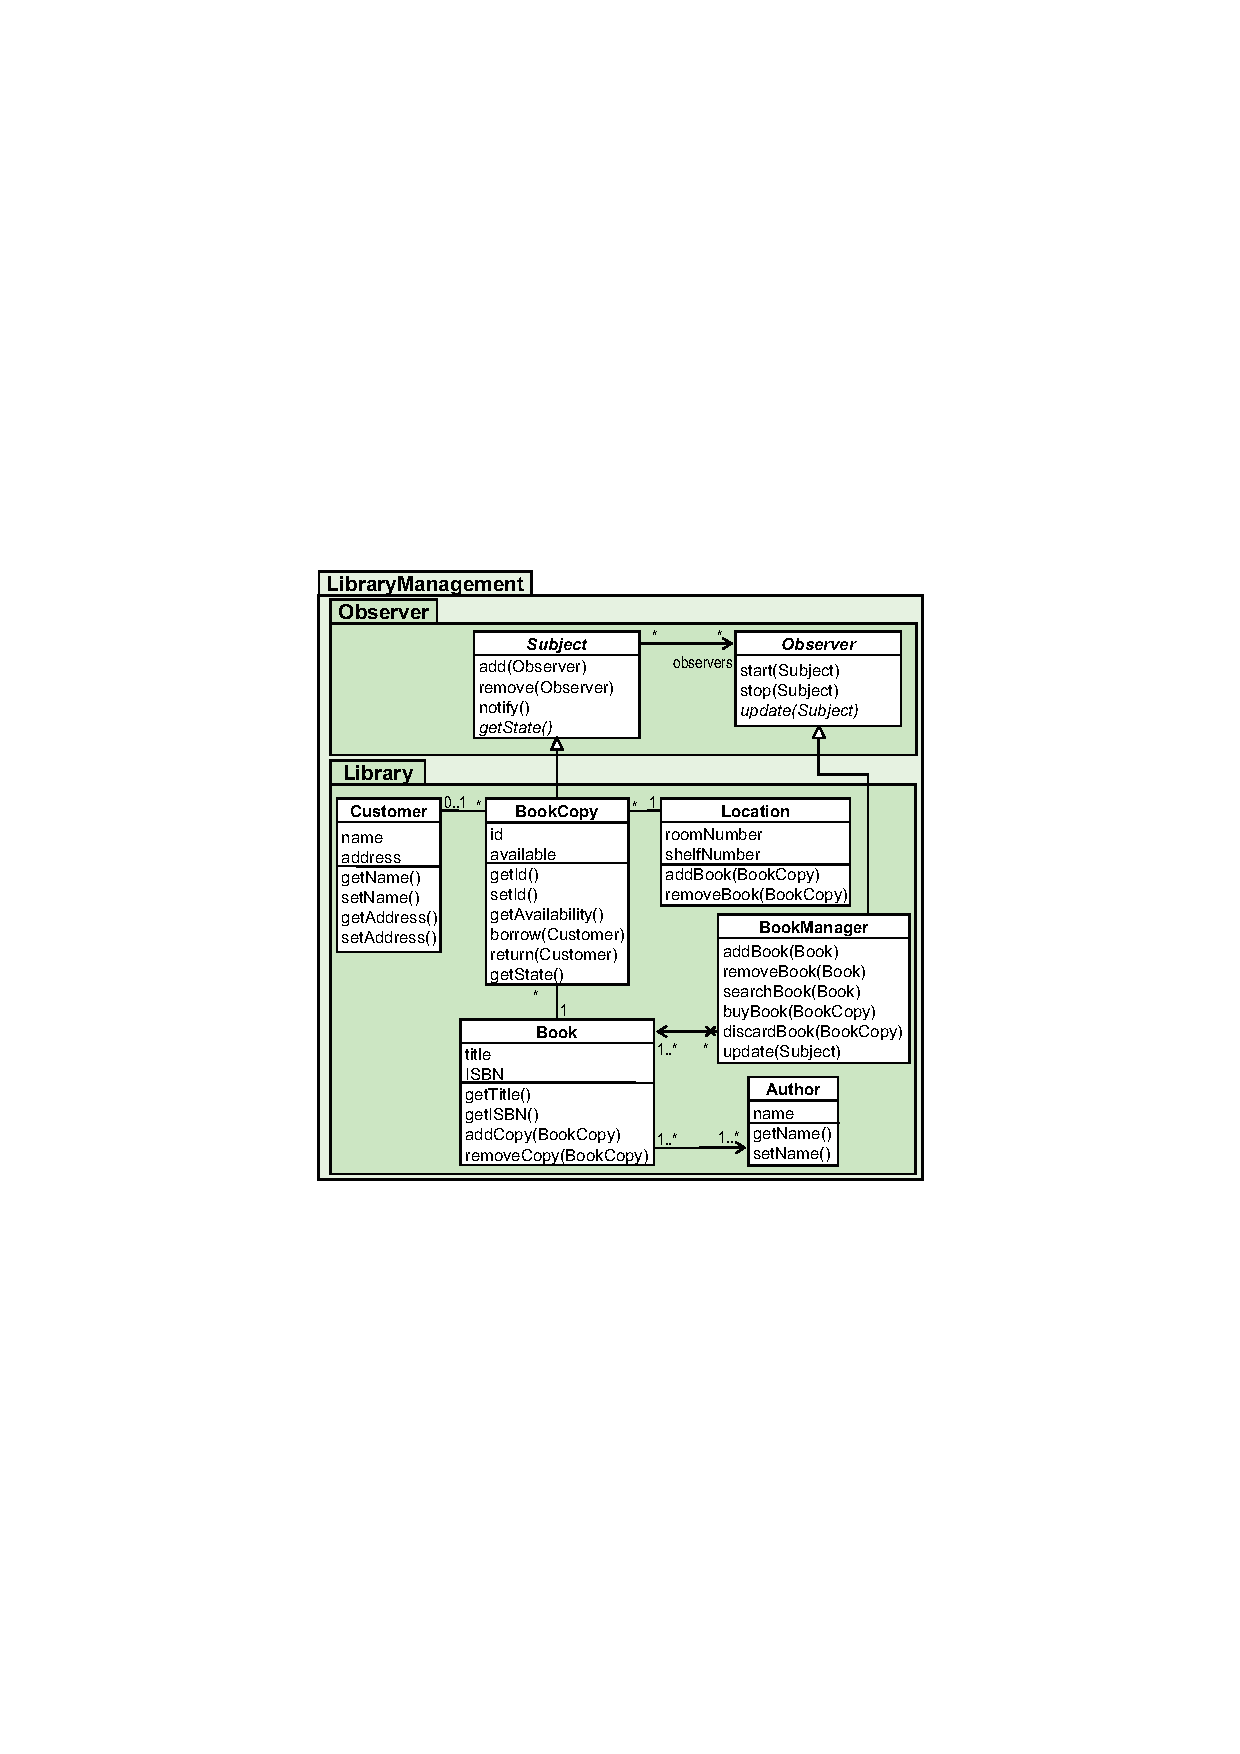
\includegraphics[width=0.7\textwidth]{figures/figure1}
%	\caption{Sample figure}
%	\label{fig:samplefigure_pdf}
%\end{figure}
%
%
%\subsection{Fonts}
%
%When introducing important terms for the first time use \emph{emphasize}. For a consistent look and feel of proper names like {\cd} and {\uml{Observer}} pattern you may define macros in the main document \texttt{thesis.tex}.
%
%\subsection{Code}
%
%For short code fragments use the \textit{verbatim} environment.
%
%\begin{verbatim}
%//Start Program
%System.out.println("Hello World!");
%//End Program
%\end{verbatim}
%
%A much better alternative is the \textit{algorithm} environment (cf. Algorithm~\ref{alg:samplealgorithm}). This environment offers special formatting features for loops, operations and comments.
%
%\begin{algorithm}[t]
%\SetKwData{Left}{left}
%\SetKwData{This}{this}
%\SetKwData{Up}{up}
%\SetKwFunction{Union}{Union}
%\SetKwFunction{FindCompress}{FindCompress}
%\SetKwInOut{Input}{input}
%\SetKwInOut{Output}{output}
%
%\Input{A bitmap $Im$ of size $w\times l$}
%\Output{A partition of the bitmap}
%
%\BlankLine
%
%\emph{special treatment of the first line}\;
%\For{$i\leftarrow 2$ \KwTo $l$}{
%\emph{special treatment of the first element of line $i$}\;
%\For{$j\leftarrow 2$ \KwTo $w$}{\label{forins}
%\Left$\leftarrow$ \FindCompress{$Im[i,j-1]$}\;
%\Up$\leftarrow$ \FindCompress{$Im[i-1,]$}\;
%\This$\leftarrow$ \FindCompress{$Im[i,j]$}\;
%\If(\tcp*[r]{O(\Left,\This)==1}){\Left compatible with \This}{\label{lt}
%\lIf{\Left $<$ \This}{\Union{\Left,\This}}\;
%\lElse{\Union{\This,\Left}\;}
%}
%\If(\tcp*[r]{O(\Up,\This)==1}){\Up compatible with \This}{\label{ut}
%\lIf{\Up $<$ \This}{\Union{\Up,\This}}\;
%\tcp{\This is put under \Up to keep tree as flat as possible}\label{cmt}
%\lElse{\Union{\This,\Up}}\tcp*[r]{\This linked to \Up}\label{lelse}
%}
%}
%\lForEach{element $e$ of the line $i$}{\FindCompress{p}}
%}
%\caption{Sample algorithm}\label{alg:samplealgorithm}
%\end{algorithm}
%
%\section{Bibliographic Issues}
%
%\subsection{Literature Search}
%
%Information on online libraries and literature search, e.g., interesting magazines, journals, conferences, and organizations may be found at \url{http://www.big.tuwien.ac.at/teaching/info.html}.
%
%\subsection{BibTeX}
%
%BibTeX should be used for referencing.
%
%The LaTeX source document of this pdf document provides you with different samples for references to journals~\cite{jour:B2BServices}, conference papers~\cite{proc:TheWebMLApproach}, books~\cite{book:umlatwork}, book chapters~\cite{incoll:ErhardKonrad1992}, electronic standards~\cite{man:BPEL}, dissertations~\cite{phdthesis:manuelWimmer}, masters' theses~\cite{mast:AUMLProfile}, and web sites~\cite{misc:BIGWebsite}. The respective BibTeX entries may be found in the file \texttt{references.bib}. For administration of the BibTeX references we recommend \url{http://www.citeulike.org} or JabRef for offline administration, respectively.

\bibliographystyle{acm}
\bibliography{references}

\end{document}
